\section{Stat Phys of photon gas}

    \begin{frame}{Spazio delle fasi del sistema, stati microscopici, evoluzione}%
\begin{itemize}
    \item Macroscopic properties are ensemble average
    \item Macroscopic evolution: flow of density of states in PS (fluid is the large collection of identical systems in same macroscopic state)
    \item Microstate probability: $\#\text{ of states}=\rho(p,q)\,dp\,dq$
    \item Isolated System is in equilibrium iff accessible microstates are equiprobable
\item Ergodic system: trajectory in phase space are deterministic ($\dot{p}_i=-\PDy{q_i}{H}$, $\dot{q}_i=\TDy{p_i}{H}$) and starting from a point will get arb. closer to any other points.
\item Evolution of systems starting inside a small cube in phase space is described with $\TDy{t}{\rho}=\PDy{t}{\rho}+\{\rho,H\}=0$ preserve volume ($\TDof{t}(x+\delta x)=\dot{x}+\delta x\PDof{x}\dot{x}$,$\TDof{t}(p+\delta p)=\dot{p}+\delta p\PDof{p}\dot{p}$ quindi $\dot{V}=\delta x\delta p[\PDof{p}\dot{p}+\PDof{x}\dot{x}]=0$). Per sistemi in equilibrio termodinamico le medie non dipendono esplicitamente dal tempo quindi neanche $\rho(p,q)$: $\{\rho,H\}=0$.
\item Microcanonical ensemble: a particular solution is $\rho(p,q)=\const{}$ (all microstates accessible between $E$,$E+\delta E$, V and N are equiprobable)
\item Canonical ensemble: system in thermal bath at T $\rho(p,q)=\exp{-\frac{H(p,q)}{kT}}$, fixed V, N and T.
\item Gran-canonical ensemble: system in thermal/chemical equilibrium with reservoir, ie fixed T,$\mu$; $\rho(p,q)\propto\exp{-\frac{H(p,q)}{kT}}\exp{+\frac{\mu N}{kT}}$.
\item $d\omega=\frac{d^{3N}p\,d^{3N}q}{(2\pi\hbar)^N}$: $S(U)=k\ln{\Omega(U)}$, $\Omega(U)$ is volume PS $H(p,q)\leq U$
\end{itemize}
\end{frame}

\begin{frame}{Gas di fotoni: Ensemble canonico.}
    \begin{itemize}
        \item Microcanonical (NVE):
        $W=\exp{\frac{S}{k}}$ numero di stati microscopici tra $E$,$E+\Delta E$, $U=\exv{H}=E(S,V,N)$.
    \item Canonical: fixed T, partition function $Z(\beta)=\sum_{\substack{k\text{ microstates}:\\\text{V,N fixed}}}\exp{-\beta E_k}=\sum_{\text{Energies }i}g_i\exp{-\beta E_i}$.
        \begin{align*}
            &\exv{U}=-\PDof{\beta}\ln{Z_{CAN}}=\sum_s\frac{\sum_{n_s}n_sh\nu_s\exp{-\theta\sum_sn_sh\nu_s}}{\sum_{n_s}\exp{-\theta\sum_sn_sh\nu_s}}=-\sum_s\PDof{\theta}\ln{\sum_{n_s}\exp{-\theta n_sh\nu_s}}\\
&=\sum_s\frac{h\nu_s}{\exp{\theta h\nu_s}-1}\xrightarrow{\vec{k}=\frac{2\pi}{L}\vec{n}}\frac{8\pi V}{c^3}\int_0^{\infty}\frac{h\nu^3}{\exp{\frac{h\nu}{kT}}-1}\,d\nu\\
&\frac{U}{V}=\frac{4\sigma}{c}T^4=aT^4
\end{align*}
$F=U-TS$: processo isotermo rev., $\Delta Q$ system, $\Delta W=P\Delta V$ work to world; $\Delta U=\Delta Q-P\Delta V$, $\Delta S=\frac{\Delta Q}{T}$ quindi $P=-\frac{\Delta U-T\Delta S}{\Delta V}\to-\frac{\Delta F}{\Delta V}|_{T,N}$, $F=-\frac{4\sigma}{3c}VT^4=-kT\ln{Z}=KT\sum_{\vec{k},\gamma}\ln{[1-\exp{-\beta\omega\hbar}]}$
    \end{itemize}
\end{frame}

%\begin{multicols}{2}%https://newbedev.com/how-to-explicitly-split-long-toc-in-beamer
%   \tableofcontents[currentsection]{cherryframes}
%\end{multicols}


\begin{wordonframe}{Relazione tra $P(\rho, T)$: approx zero gas perfetto di atomi completamente ionizzati}
\begin{columns}[]%
    \hspace{-19pt}\relax
\begin{column}{0.55\textwidth}%
EOS gas perfetto di ioni ed elettroni 
\begin{equation*}
P_G=P_I+P_e=\frac{\rho}{\mu}\gasconstant{}T
\end{equation*}
Energia interna per unit\'a di massa: somma delle energie traslazionali delle particelle pesate secondo la distribuzione di equilibrio di Maxwell-Boltzmann per grammo di materia
\begin{align*}
&u=\frac{1}{\rho}\sum_i\int f^{(0)}(\vec{p}_i)\frac{p^2_i}{2m_i}\,d^3p_i\\
&=\frac{3}{2}\frac{P}{\rho}=\frac{3}{2}\frac{\gasconstant T}{\mu}
\end{align*}
\end{column}
    \hspace{-22pt}\relax
\begin{column}{0.45\textwidth}
Peso molecolare medio: massa media in amu per particella libera
\begin{align*}
&\mu=\frac{1}{\bar{n}_HX+\bar{n}_{He}Y+\bar{n}_{Z}Z}\\
&\mu_0=\frac{1}{X+\midfrac{Y}{4}+\midfrac{Z}{\bar{A}}},\ \mu_e\approx\frac{2}{1+X}
\end{align*}
con $\bar{n}_i=\frac{1+f_i}{A_i}$ numero medio di particelle libere per unit\'a di massa atomica dovute alla specie i di peso atomico $A_i$ e $f_i$ numero medio di elettroni liberati da ione della specie i; peso atomico medio per ione $\mu_0$ ed elettrone libero (ionizzato) $\mu_e$.
\end{column}
\end{columns}
$f^{(0)}(\vec{p}_i)$: numero di particelle della specie i per unit\'a di volume con impulso in $[\vec{p}_i,\vec{p}_i+d\vec{p}_i]$
\end{wordonframe}

\begin{wordonframe}{Deviazioni dalla legge dei gas perfetti: radiazione e degenerazione elettronica}
\begin{itemize}
	\item Radiazione. Il contributo alla pressione ed energia interna per unit\'a di volume dei fotoni $P_R=\frac{a}{3}T^4$, $u_R=aT^4$, e $P-P_R=\beta P$.
	\item Degenerazione elettronica - Principio di Pauli: non pi\'u di 2 elettroni in volume di spazio delle fasi $h^3$. $n_e$ la densit\'a numerica di \Pelectron, $\psi(P,T)$ il parametro di degenerazione, tale che per $\psi\to-\infty$ si abbia la distribuzione di Boltzmann e per $\psi\to+\infty$ completa degenerazione
	\begin{align*}
	&n_e=\rho N_A\frac{1+X}{2}=\intzi{}\frac{8\pi p^2\,dp}{h^3(\exp{\frac{u_k}{KT}-\psi}+1)}=\frac{8\pi}{h^3}(2m_ekT)\expy{3/2}a(\psi)\\
	&P_e=\beta P-\rho\gasconstant{}(X+\frac{Y}{4}+\frac{Z}{\exv{A_Z}})=\frac{8\pi}{3h^3}\intzi{}p^3v(p)\frac{dp}{1+\exp{\epsilon/kT-\psi}}\\
	&U_e=\frac{8\pi}{h^3}\int_0^{\infty}\frac{p^2\epsilon(p)\,dp}{\exp{(-\psi+\midfrac{\epsilon}{KT})}+1}
	\end{align*}
\end{itemize}
\end{wordonframe}

\begin{frame}{degenerazione completa: casi limite NR e R}
\begin{align*}
&P_e=\int_{2\pi}\frac{d\Omega}{4\pi}\intzi{}dpf(p)v(p)p^2\cos{\theta}=\frac{8\pi}{3h^3}\int_0^{P_F}p^3v(p)\,dp\\
&=\frac{8\pi c}{3h^3}\int_0^{P_F}\frac{p/(m_ec)}{\sqrt{1+p^2/(m_ec)^2}}=\frac{\pi m_e^4c^5}{3h^2}f(x)\\
&U_e=\int_0^{P_F}f(p)E(p)\,dp=\frac{8\pi}{h^3}\int_0^{P_F}E(p)p^2\,dp=\frac{\pi m_e^4c^5}{3h^3}g(x)\
\end{align*}
\begin{align*}
&n_e=\frac{\rho}{\mu_em_H}=\frac{8\pi m_ec^3}{3h^3}x^3\\
&x=\frac{P_F}{m_ec}\ll1:\quad&x\gg1:\\
&P_e=\frac{8\pi m_e^4c^5}{15h^3}x^5=\frac{2}{3}U_e&P_e=\frac{2\pi m_e^4c^5}{3h^3}x^4=\frac{1}{3}U_e\\
&=\num{1.0036e13}(\frac{\rho}{\mu_e})\expy{5/3}&=\num{1.2435e15}(\frac{\rho}{\mu_e})\expy{4/3}
\end{align*}
\end{frame}

\begin{wordonframe}{Elettrostatic screening of ions: weak screening}
La principale correzione che tiene conto dell'interazioni tra particelle \'e dovuta alle interazioni coulombiane: influence EOS and nuclear rection rates.

Screening of ion i with charge $Z_ie$ ar $\vec{r_i}$ in NR dilute plasma, motion of screened ions is slow compared to screening particles: continuum static equilibrium charge distribution (\Pelectron, light ions of mean charge $Z_p$)
\begin{equation*}
\nabla^2\phi=4\pi n_ee[\exp{(\frac{e\phi}{kT})}-\exp{-\frac{Z_pe\phi}{kT}}]-4\pi\sum_iZ_ie\delta(\vec{r}-\vec{r_i})
\end{equation*}
Regime di schermaggio debole, $e\phi\ll KT$: $\phi=\sum_i\phi_i$ potenziale attorno a ione pesante isolato:
\begin{align*}
%&\nabla^2\phi=-4\pi e\sum_Z Zn_Z-4\pi e\sum_i Z_i\delta(\vec{r}-\vec{r}_i)\\
&\phi_i=\frac{Z_ie}{r_i}\exp{-\frac{r_i}{r_D}}
&\frac{1}{r_D^2}=\frac{4\pi e^2}{kT}\sum Z^2\overline{n}_Z=\frac{4\pi e^2}{kT}N_A\zeta,\ \zeta=\sum_{i}(Z_i^2+Z_i)\frac{\rho X_i}{A_i}
\end{align*}
\end{wordonframe}

\begin{wordonframe}{Elettrostatic screening of ions: energy pressure correction}
Energy required to assemble uniform shere with charge $Ze$: $U_{ee}=\int_0^{R_Z}\frac{q_r}{r}\,dq=\frac{3}{5}\frac{(Ze)^2}{R_Z}$.
Energy required to assemble uniform cloud of charge $Ze$ around Z-nucleus: $U_{eZ}=-Ze\int_0^{R_Z}\frac{dq}{r}=-\frac{3}{2}\frac{(Ze)^2}{R_Z}$
Le correzioni dovute alle interazioni coulombiane sono dovute a numero sfere ioniche per unit\'a di volume $n_Z=\frac{\rho X_Z}{A_Z}N_0$ with average potential energy per electron $\exv{-e\phi}_Z=-\frac{9}{10}\frac{(Ze)^2}{R_Z}$ that contain Z \Pelectron.
\begin{align*}
&\rho u_c=(\frac{U}{V})_e=\frac{1}{2}\phi(\vec{r})\rho_c(\vec{r})\to \frac{1}{2}\sum_ZeZ\overline{n}_Z\phi_Z=-e^3\sqrt{\frac{\pi\rho}{kT}}(N_A\zeta)\expy{\frac{3}{2}},\ P_c=\frac{1}{3}\rho u_c\\
&E_0=\frac{(U/V)_e}{n_e}=\mu_e\sum_Z\exv{-e\phi}_Z\frac{ZX_Z}{A_Z}\approx-1.3(\mu_e^2\rho)\expy{1/3}[X+0.79Y+\sum_{Z>2}\frac{Z\expy{5/3}X_Z}{A_Z}]
\end{align*}
\end{wordonframe}

\begin{frame}{Equazione di Saha e continuum depression. Ioniozzazione da pressione}
L'equazione di Saha descrive la frazione relativa di ionizzazione
\begin{align*}
&\frac{n_{r+1}}{n_r}n_e=\frac{g_{r+1}}{g_r}f_r(T)\\
&f_r(T)=2\frac{(2\pi m_ekT)\expy{3/2}}{h^3}\exp{-\chi_r/(kT)}
\end{align*}
Saha limitation:
\begin{itemize}
\item LTE: is the case when collision dominate over radiative processes
\item Decreases ionization energy with increasing density: what is called pressure ionizzation is produced by coulomb interaction of bound electron with other electron in the plasma $\chi'_Z=\chi_Z-\frac{Ze^2}{R_D}$
\end{itemize}
\end{frame}

\section{Radiative transfer equation}

\begin{frame}{Derivation of transfer equation}
    \begin{columns}[T]
        \begin{column}{0.3\textwidth}
\begin{figure}[!ht]
	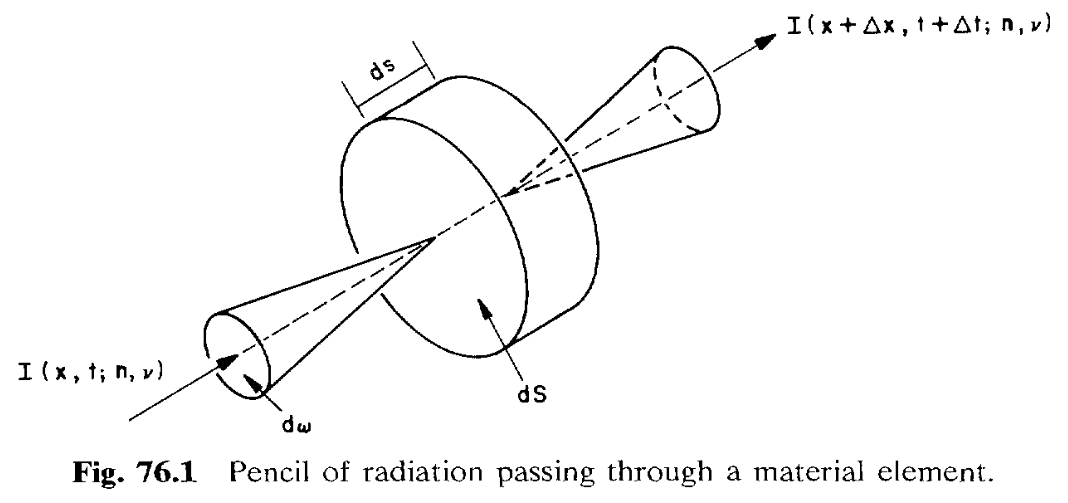
\includegraphics[trim={0cm 0cm 1cm 0cm},clip, keepaspectratio,width=0.99\textwidth]{radthroughcyl}
\end{figure}
        \end{column}
        \begin{column}{0.7\textwidth}
\begin{align*}
    &\Delta t=\frac{ds}{c}:\ I(\vec{x}+\Delta\vec{x},t+\Delta t;\vec{n},\nu)\\
    &=I(\vec{x},t;\vec{n},\nu)+[\frac{1}{c}\PDy{t}{I}]\,ds
\end{align*}
        \end{column}
    \end{columns}
  \begin{align*}
   &I(\vec{x}+\Delta\vec{x},t+\Delta t;\vec{n},\nu)-I(\vec{x},t;\vec{n},\nu)=[\eta(\vec{x},t;\vec{n},\nu)-\chi(\vec{x},t;\vec{n},\nu)I(\vec{x},t;\vec{n},\nu)]ds\,dS\,d\Omega\,d\nu\,dt&\\
   &[\frac{1}{c}\PDof{t}+\nabla_{\vec{s}}]I(\vec{x},t;\vec{n},\nu)=\eta(\vec{x},t;\vec{n},\nu)-\chi(\vec{x},t;\vec{n},\nu)I(\vec{x},t;\vec{n},\nu)&\tag{Trans. eq.}\\
   &[\frac{1}{c}\PDof{t}+\mu\PDof{z}]I(z,t;\mu,\nu)=\eta(z,t;\mu,\nu)-\chi(\ldots)I(\ldots)&\tag{1D planar}
  \end{align*}

  \begin{columns}[T]
      \begin{column}{0.15\textwidth}
          \begin{figure}[!ht]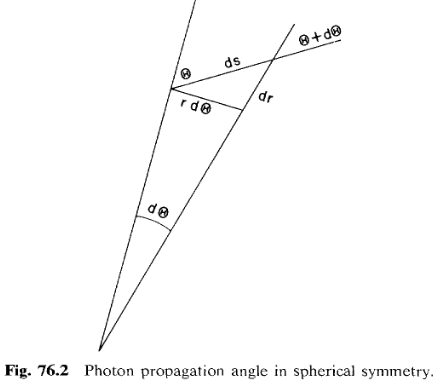
\includegraphics[trim={2cm 0cm 1cm 5mm},clip, keepaspectratio,width=0.99\textwidth]{radtransfspheric}\label{fig:}\end{figure}
      \end{column}
      \begin{column}{0.85\textwidth}
          \begin{align*}
          &dr=\cos{\Theta}\,ds=\mu\,ds,\ r\,d\Theta=-\sin{\Theta}\,ds=-\sqrt{1-\mu^2}\,ds&\tag{spherical sym}\\
          &\PDof{s}=\PDy{s}{r}\PDof{r}+\PDy{s}{\Theta}=\mu\PDof{r}+\frac{(1-\mu^2)}{r}\PDof{\mu}&\\
          &[\frac{1}{c}\PDof{t}+\mu\PDof{r}+\frac{(1-\mu^2)}{r}\PDof{\mu}]I(r,t;\mu,\nu)=\eta(r,t;\mu,\nu)-\chi(r,t;\mu,\nu)I(r,t;\mu,\nu)&
          \end{align*}
      \end{column}
  \end{columns}
  Classical, macroscopic, phenomenological: not included polarization, dispersion, coherence, interference and quantum effects.
\end{frame}

\begin{frame}{Einstein relations}
    \begin{columns}[T]
        \begin{column}{0.5\textwidth}
            Radiative transition $i\to j$: $h\nu_{ij}=\epsilon_j-\epsilon_i$, stat. weight $g_i, g_j$, \keyword{absorption probability $B_{ij}$}, \keyword{spontaneus emission probability $A_{ji}$}: isotropic
                        \[\dot{E}_{\nu}=\frac{A_{ji}h\nu_{ji}}{4\pi}n_i\phi_{\nu}\]
                \begin{align*}
                &(\frac{n_i}{n_j})^*B_{ij}I_{\nu}^*=A_{ji}+B_{ji}I_{\nu}^*\label{CR and TE}\\
                                &(\frac{n_j}{n_i})^*=\frac{g_j}{g_i}\exp{-h\nu/KT}\\
                            &\Rightarrow B_{\nu}=\frac{A_{ji}}{B_{ji}}\invers{[\frac{g_iB_{ij}}{g_jB_{ji}}\exp{h\nu_{ij}kT}-1]}\\
                        &g_iB_{ij}=g_jB_{ji}\tag{Atomic prop $\to$ E. coeff}\\
                    &A_{ji}=\frac{2h\nu_{ij}^3}{c^2}B_{ji}\tag{also for non TE}
            \end{align*}
        \end{column}
        \begin{column}{0.5\textwidth}
            Number of photons absorbed per unit volume per unit time:
            \[r_{ij}=n_i\phi_{\nu}B_{ij}I_{\nu}(\frac{d\Omega}{4\pi})d\nu\]
            \keyword{Induced emission probability $B_{ji}$}: rate of stimulated energy emission per unit volume (as $I_{\nu}$)
            \[\dot{E}_{\nu}=\frac{B_{ji}h\nu_{ij}}{4\pi}n_i\phi_{\nu}I_{\nu}\]
            \keyword{Line emission/absorption ceff} (co-moving frame):
            \begin{align*}
    &\eta_l(\nu)=n_j\frac{A_{ji}h\nu_{ij}}{4\pi}\phi_{\nu}\\
    &\chi_l(\nu)=\frac{n_iB_{ij}h\nu_{ij}}{4\pi}[1-\frac{g_in_j}{g_jn_i}]\phi_{\nu}
            \end{align*}
        \end{column}
    \end{columns}
    \begin{columns}[T]
        \begin{column}{0.4\textwidth}
             Source function for a line: ratio emissivity to opacity:
        \end{column}
        \begin{column}{0.6\textwidth}
            \[S_l=\frac{n_jA_{ji}}{n_iB_{ij}-n_jB_{ji}}=\frac{2h\nu_{ij}^3}{c^2}\invers{[\frac{g_jn_i}{g_in_j}-1]}\to B_{\nu}\]
        \end{column}
    \end{columns}
\end{frame}

\begin{frame}{Einstein-Milne relations}
    \begin{columns}[T]
        \begin{column}{0.55\textwidth}
            Fluid frame; $n_e(v)$ maxwellian - prob. ionization by rad $(\nu,\nu+d\nu)$: Energy absorption coeff. $\alpha_{\nu}=h\nu p_{\nu}$,
            photoionization rate: $n_0h\nu I_{\nu}\,d\nu$, $n_0$ atoms number density, $n_1$ density of ions - $F(v)$/$G(v)$ spontaneous/induced recombination prob for \Pelectron with $(v,v+dv)$, recombination rate: $n_1n_e(v)[F+GI]vdv$
        \end{column}
        \begin{column}{0.45\textwidth}
            Thermodynamic equilibrium: photoionizations equal recombinations
            \begin{align*}
                &n_0^*p_{\nu}B_{\nu}=n_1^*n_e(v)[F(v)+G(v)B_{\nu}]\\
                &\Rightarrow B_{\nu}=\frac{F(v)}{G(v)}\invers{(\frac{n_0^*p_{\nu}m_e}{n_1^*n_e(v)hG(v)}-1)}\\
                &\left\{\begin{array}{l}F(v)=\frac{2h\nu^3}{c^2}G(v)\\\frac{p_{\nu}}{G(v)}\frac{h}{m}[n_2(v)(\frac{n_1}{n_0})^*]\exp{h\nu/kT}\\
                \end{array}\right.\tag{1}
            \end{align*}
        \end{column}
    \end{columns}
    \begin{align}
        &n_e(v)\,dv=n_e[\frac{m_e}{2\pi kT}]^{3/2}\exp{-\frac{1}{2}\frac{mv^2}{kT}}4\pi v^2\,dv\tag{TE: $n_e$ maxwell.}\\
        &(\frac{n_1}{n_0})^*=(\frac{g_0}{2g_1})[\frac{h^2}{2\pi m_ekT}]^{3/2}\exp{\epsilon_{ion}/kT}=n_e\phi_0\tag{Saha eq.}\\
        &\Rightarrow p_{\nu}=\frac{8\pi m^2v^2g_1}{h^2g_0}G(v)=\frac{4\pi c^2m^2v^2g_1}{h^3g_0\nu^3}F(v)\tag{2}
    \end{align}
 (1)-(2) continuum analog of Einstein relations   
\end{frame}

\begin{frame}{Continuum emission/absorption coeff.}
    \begin{align*}
        &\kappa_{\nu}=h\nu[n_0p_{\nu}-\frac{h}{m}n_1n_e(v)G(v)]=[n_0-n_0^*\exp{-\frac{h\nu}{kT}}]\alpha_{\nu}\\
        &\kappa_{\nu}^*=n_0^*\underbrace{[1-\exp{-\frac{h\nu}{kT}}]}_{\text{correction stimulated emission}}\alpha_{\nu}\tag{LTE}
    \end{align*}
    Recombination (spontaneous/induced) results from ion-electrons collision: if they have Maxwellian distribution, recombination at LTE rate whereas for lines rate depends on upper level population - Spontaneous continuum emission coeff.:
\begin{align*}
    &\eta_{\nu}^t=h\nu n_1n_e(v)F(v)\frac{h}{m}=\frac{hn_1n_e(v)F(v)}{m_ep_{\nu}}\alpha_{\nu}\\
    &\to\frac{2h\nu^3}{c^2}n_0^*\alpha\exp{-\frac{h\nu}{kT}}=n_0^*(1-\exp{-\frac{h\nu}{kT}})\alpha_{\nu}B_{\nu}(T)=\kappa_{\nu}^*B_{\nu}(T)
\end{align*}
\end{frame}

\begin{frame}{Absorption, emission and scattering}
    \begin{itemize}
        \item \keyword{Total absorption coef $\chi(\vec{x},t;\hat{n},\nu)$}: material volume of cross section $dS$ and length $dl$ removes energy from beam in interval dt:
            \[\delta=\chi(\ldots)I(\ldots)dld\Omega d\nu dt\]
            Sum over all states that can absorb at $\nu$ of the product of occupation number of those states (\si{\per\cubic\cm}) times their atomic crosssection (\si{\square\cm}) at that freq.: $\lambda_{\nu}=\invers{\chi_{\nu}}$ is mean free path of photons
        \item \keyword{Doppler Shift}: Photons moving along $\hat{n}$ with freq. $\nu$ in Lab. frame, has in fluid frame of materials moving at $\vec{v}$ freq. $\nu_0=\nu[1-\frac{\vec{v}\cdot\hat{n}}{c}]$ ($\frac{\Delta\nu_D}{\nu_0}c=13(\frac{T}{\SI{e4}{\kelvin}})^{1/2}\si{\kilo\meter\per\second}$).
        \item \keyword{Emission coeff. (Emissivity)}: $\eta(\vec{x},t;\hat{n},\nu)$ such that an element $dS\,dl$ add energy to beam
            \[\delta E=\eta(\ldots)dldSd\Omega\,dVdt\ [\si{\erg\per\cubic\cm\per\second\per\hertz\per\ster}]\]
        \item \keyword{Scattering}: Photon excites atoms then atoms decay into fundamentals - Photons collides with free electrons (Thopson scattering), atom or molecule in which they excite a resonance (Rayleigh/Raman scattering) 
    \end{itemize}
\end{frame}

\begin{frame}{Kirchoff-Plank relation}
    In TE: $(\eta_{\nu}^t)^*=(\kappa_{\nu}I_{\nu})^*$, $*$ indica TE dove $I_{\nu}=B_{\nu}$ quindi $(\eta_{\nu}^t)^*=(\kappa_{\nu}B_{\nu})^*$ - when gradients of physical quantities are small over photon destruction lenght: LTE
\end{frame}

\begin{frame}{Thermodynamics of adiabat enclosed rad: Kirchoff-Plank rel.}
    \begin{block}{Einstein coeff.}
Radiative transition $i\to j$: $h\nu_{ij}=\epsilon_j-\epsilon_i$, stat. weight $g_i, g_j$, \keyword{absorption probability $B_{ij}$}, \keyword{spontaneus emission probability $A_{ji}$}: isotropic
            \[\dot{E}_{\nu}=\frac{A_{ji}h\nu_{ji}}{4\pi}n_i\phi_{\nu}\]
            \begin{align*}
                &(\frac{n_i}{n_j})^*B_{ij}I_{\nu}^*=A_{ji}+B_{ji}I_{\nu}^*\label{CR and TE}\\
                &(\frac{n_j}{n_i})^*=\frac{g_j}{g_i}\exp{-h\nu/KT}\\
                &\Rightarrow B_{\nu}=\frac{A_{ji}}{B_{ji}}\invers{[\frac{g_iB_{ij}}{g_jB_{ji}}\exp{h\nu_{ij}kT}-1]}\\
                &g_iB_{ij}=g_jB_{ji}\tag{Atomic prop $\to$ E. coeff}\\
                &A_{ji}=\frac{2h\nu_{ij}^3}{c^2}B_{ji}\tag{also for non TE}
            \end{align*}
   \end{block}
   \begin{block}{E. of transfer in star interior}
       \begin{align}
        &\TDy{s}{I_{\nu}}\frac{1}{\rho}=j_{\nu}-\kappa_{\nu}I_{\nu}\Leftrightarrow\TDy{s}{I_{\nu_{nm}}}=N_n(A_{nm}+B_{nm}I_{\nu_{nm}})h\nu_{nm}-N_mB_{mn}h\nu_{nm}I_{\nu_{nm}}\label{ERT}
    \end{align}
    \begin{columns}[T]
        \begin{column}{0.3\textwidth}
            $I_{\nu}$ in isotropic homogeneous medium adiabat. enclosed deps only on T:
        \end{column}
        \begin{column}{0.7\textwidth}
        \begin{align*}
        \frac{1}{\rho}\TDy{s}{I_{\nu}}=0\Rightarrow j_{\nu}=\kappa_{\nu}I_{\nu}\Rightarrow I_{\nu_{nm}}=\frac{N_nA_{nm}}{N_mB_{mn}-N_nB_{nm}}\label{Kirckoff-Plank}
\end{align*}
        \end{column}
    \end{columns} 
   \end{block}
\end{frame}
\begin{frame}{Scattering of radiation in spectral line}
    \begin{itemize}
    \item Broadened atomic level can be decomposed into sublevels and transition between these sublevels can be treated statistically: \keyword{redistribution function}: probability in atom's frame that incoming photon of freq $\nu'$ is scattered as outgoing $\nu$.
    \item Semiclassical picture
    \item Natural population of levels: probability emitting photon $(\hat{n},\nu)$ in transition to lower level averaged over ensemble of identical atoms is independent of previous history of ensemble (not naturally populated by radiative processes in which there is correlation with prop. prev. absorbed/emitted photon: stimulated emission)
\item Distro of individual sublevel of naturally popul. n at $E_n$: $L(\chi,\gamma)=\frac{\gamma}{\pi(\chi^2+\gamma^2)}$, $\chi=\frac{E-E_n}{h}$, $2\gamma_n=\sum_{m<n}A_{nm}+\sum_{m\neq n}B_{nm}\bar{J}_{nm}+R_{n\kappa}+\sum_{n\neq m}C_{nm}+C_{n\kappa}+Q_n$, A,B bb Einstein coeff., R photoion rate, C coll rate (bb,bf), $Q_n$ effective rate of elastic coll.in level n, $\bar{J}_{nm}=\int_0^{\infty}\oint \frac{d\Omega}{4\pi}\phi_{nm}(\nu,\hat{n})\,d\nu$ freq-averaged mean intensity for $n\to m$ (suppose spont em coeff much bigger than induced em coeff)
\item Atom's frame absorption profile for transition between broadened level $i\to e$: $\phi_{ie}(\nu')=\intsinf{}L(\chi_i,\gamma_i)L(\chi_e',\gamma_e)\,d\chi_i$; $L(\chi_i,\gamma_i)$ natural occupation probability of sublevels in $(\chi_i,\chi_i+\,d\chi_i)$, $L(\chi_e'=\nu'-\nu_{ie}+\chi_i,\gamma_e)$ is occupation prob of level e when photon $\nu'$ is absorbed, total prob of transition is product summed over all i states, Cauchy's residue theorem $\phi_{ij}(\nu')=L(\nu'-\nu_{ij},\gamma_{ij})=\frac{\gamma_{ij}}{\pi[(\nu'-\nu_{ij})^2+\gamma_{ij}^2]}$, $\gamma_{ij}=\gamma_i+\gamma_j$
\end{itemize}
\end{frame}

\begin{frame}{Semiclassical picture of photon scattering}
    
\end{frame}

\section{Opacit\'a}\linkdest{kapparad}

\begin{frame}{Opacit\'a radiativa (analitico)}
Scattering elettronico, processi ff, fotoionizzazione; opacit\'a atmosfera: ione H-
\end{frame}

\begin{frame}{Andamento opacit\'a: electron scattering e Kramer's opacity (FF)}
\begin{itemize}
\item Electron scattering $\rho\kappa_{\nu}=n_e\frac{8\pi}{3}(\frac{e^2}{m_ec^2})^2=0.2(1+X)\si{\square\cm\per\gram}$ - $\sigma_T=\SI{0.66e-24}{\square\cm}$ - for $T$ maggiore di few milion K is dominant source - Compton scattering $h\nu|_M\gtrsim0.1 m_ec^2$, $h\nu|_M\approx4.96kT$: Compton scattering reduces opacity about $20\%$ for $T>\SI{e8}{\kelvin}$
\item Kramers opacity: $T<\SI{e7}{\kelvin}$ -when FF, BF dominates: $\kappa_R\propto\rho T\expy{-7/2}$
\end{itemize}
\begin{block}{Free-free: radiation boost free-\Pelectron from lower to higher state}
Fully ionized-$Z_i$ mixture: 
\begin{align*}
&\rho\kappa_{\nu}(ff)=\sum_in_{Z_i}ne\sqrt{\frac{2m_e}{3\pi kT}}[\frac{4\pi Z_i^2e^6}{3m_e^2ch\nu^3}]g_{ff}(\nu)(1-\exp{-h\nu/kT})\\
&=\num{3.8e22}\overbrace{(X+1)}^{\propto n_e}\overbrace{[X+Y+B]}^{\propto\frac{X}{m_u}+\frac{4Y}{4m_u}+\sum_i\frac{X_iZ_i^2}{A_i}}\ [\si{cgs}]
\end{align*}
$\tau_{\Pelectron-int}\propto\frac{1}{v}\propto T\expy{-1/2}$: \Pelectron experience sharp acceleration $\approx\delta$ resulting in constant emission frequency, two body ion-\Pelectron encounter $\propto n_in_e$, \Pelectron have thermal distro $\propto\exp{-\epsilon/kT}$: $\rho j_{\nu}=n_en_iT\expy{-1/2}\exp{-\frac{h\nu}{kT}}$ - dalla legge di Kirchhoff, $j_{\nu}=4\pi\kappa_{\nu}^{abs}B_{\nu}(T)$, we have $\kappa_{\nu}^{abs}\propto\rho T\expy{-1/2}\nu\expy{-3}[1-\expy{-h\nu/kT}]$
\end{block}
\end{frame}

\begin{frame}{Kramer's opacity (BF, BB) and $H^-$ ions opacity}
\begin{block}{BF}
Hydrogenic atom with charge Z and one \Pelectron in bound state n:
\begin{align*}
&\sigma_{\nu}(Z)=n\expy{-5}\frac{8\pi}{3\sqrt{3}}\frac{Z^4m_ee\expy{10}}{c\hbar^3(h\nu)^3}:\ h\nu>\chi=\frac{Ze^2}{2a_Z}\\
&\rho\kappa_{\nu}(bf)=\sum_in_{Z_i}\sigma_{\nu}(Z_i)(1-\exp{-h\nu/kT})\\
&\kappa_R(bf)=\num{3e25}\underbrace{(1-X-Y)}_{n_{\exv{Z}}}\underbrace{(1+X+\frac{3}{4}Y)}_{n_e}\rho T\expy{-7/2}
\end{align*}
\end{block}
\begin{block}{BB: usually neglected in stellar interior}
\end{block}
\begin{block}{$H^-$ opacity $T<\SIrange{e4}{e5}{\kelvin}$}
BB/BF transition for $H^-$ don't follow Kramer as ion abundance in solar photosphere is sensitive to other considerations: law of mass action for $H^-=H+\Pelectron$ is $\frac{n_{H^-}}{n_Hn_e}=K_1(T)$, and sources of free electrons are metals (Na, K) $M^++\Pelectron=M$ so $\frac{n_{M^+}n_e}{n_M}=K_2(T)$, supposing $n_e=n_{M^+}$:
\begin{align*}
&\rho\kappa_{H^-}^{ff}\propto n_{H^-}n_eT\expy{-7/2}=n_Hn_MT\expy{-7/2}K_1(T)K_2(T)
\end{align*}
\end{block}
\end{frame}

\begin{frame}{True absorption and scattering coeff.}
    True absorption plus scattering $\chi=\kappa+\sigma$, thermal emission plus scattering emission $\eta=\eta^T+\eta^S$ - if $\sigma_l$ (line scattering cross section) is isotropic total energy removed from beam is
    \begin{align*}
        &\sigma(\ldots)\intzi\,d\nu_0'\phi(\vec{x},t;\nu_0')\oint\,d\Omega_0'I_0(\vec{x},t;\hat{n}_0',\nu_0')\\
        &=4\pi\sigma_l(\vec{x},t)\intzi\phi(\vec{x},t;\nu_0')J_0(\vec{x},t;\nu_0')d\nu_0'
    \end{align*}
    Prob. absorption of photon with $(\hat{n}',\nu')$ absorbed and re-emitted on $(\hat{n},\nu)$ is $R(\hat{n}',\nu',\hat{n},\nu)$.
    If photons are random in angle and along line profile (\keyword{complete redistribution}: good approx. in many cases, within Doppler core of a line, if excited atoms suffer many collisions before re-emission) the fluid frame/lab. frame emission(emissivity) by scattering is
    \begin{align*}
        &\eta_0^S(\vec{x},t;\nu_0)=\sigma(\ldots)\phi(\vec{x},t;\nu_0)\intzi\,d\nu_0'\phi(\vec{x},t;\nu_0')J_0(\vec{x},t;\hat{n}_0',\nu_0')\\
        &\eta^S(\vec{x},t;\hat{n},\nu_0)=\sigma(\ldots)\phi(\vec{x},t;\nu_0)\intzi\,d\nu_0'\oint\,d\Omega\phi(\vec{x},t;\nu_0')I_0(\vec{x},t;\hat{n}_0',\nu_0')
    \end{align*}
    When scattering is isotropic and coherent the emissivity is $\eta_0^S=\sigma_0(\vec{x},t)J_0(\vec{x},t;\nu_0)$: Thompson scattering of continuum photons by free electrons
\end{frame}

  \begin{frame}{Total Opacity and Total Emission coeff. and LTE}
      \begin{align*}
              &\chi_{\nu}=\kappa_{\nu}+\sigma_{\nu}=\underbrace{\sum_i\sum_{j>i}[n_i-\frac{g_i}{g_j}n_j]\alpha_{ij}(\nu)}_{\text{BB - line}}+\underbrace{\sum_i(n_i-n_i^*\exp{-\frac{h\nu}{kT}})\alpha_{ik}(\nu)}_{\text{BF}}\\
                      &+\underbrace{\sum_{\kappa}n_en_{\kappa}\alpha_{\kappa\kappa}(\nu,T)(1-\exp{-\frac{h\nu}{kT}})}_{\text{FF}}+\underbrace{n_e\sigma_e}_{\text{Thompson scatt. by free e}}\tag{Tot.Opa.}\\
          &\eta_{\nu}^{th}=\frac{2h\nu^3}{c^2}[\sum_i\sum_{j>i}n_j \frac{g_i}{g_j}\alpha_{ij}(\nu)+\sum_in_i^*\alpha_{i\kappa}(\nu)\exp{-\frac{h\nu}{kT}}+\sum_{\kappa}n_en_{\kappa}\alpha_{\kappa\kappa}(\nu,T)\exp{-\frac{h\nu}{kT}}]\\
                  &\xrightarrow{LTE}\frac{2h\nu^3}{c^2}\exp{-\frac{h\nu}{kT}}[\sum_in_i^* (\sum_{j>i}\alpha_{ij}(\nu)+\alpha_{i\kappa}(\nu))+\sum_{\kappa}n_en_{\kappa}\alpha_{\kappa\kappa}(\nu,T)\exp{-\frac{h\nu}{kT}}]\\
                          &\Rightarrow\chi_{\nu}^*=\kappa_{\nu}^*+n_e\sigma_e,\ (\eta_{\nu}^{th})^*=\kappa_{\nu}^*B_{\nu}
          \end{align*}
          \end{frame}

\section{Solution of RE in far interior}


\begin{frame}{Total Opacity and Total Emission coeff. and LTE}
    \begin{align*}
        &\chi_{\nu}=\kappa_{\nu}+\sigma_{\nu}=\underbrace{\sum_i\sum_{j>i}[n_i-\frac{g_i}{g_j}n_j]\alpha_{ij}(\nu)}_{\text{BB - line}}+\underbrace{\sum_i(n_i-n_i^*\exp{-\frac{h\nu}{kT}})\alpha_{ik}(\nu)}_{\text{BF}}\\
        &+\underbrace{\sum_{\kappa}n_en_{\kappa}\alpha_{\kappa\kappa}(\nu,T)(1-\exp{-\frac{h\nu}{kT}})}_{\text{FF}}+\underbrace{n_e\sigma_e}_{\text{Thompson scatt. by free e}}\tag{Tot.Opa.}\\
        &\eta_{\nu}^{th}=\frac{2h\nu^3}{c^2}[\sum_i\sum_{j>i}n_j \frac{g_i}{g_j}\alpha_{ij}(\nu)+\sum_in_i^*\alpha_{i\kappa}(\nu)\exp{-\frac{h\nu}{kT}}+\sum_{\kappa}n_en_{\kappa}\alpha_{\kappa\kappa}(\nu,T)\exp{-\frac{h\nu}{kT}}]\\
        &\xrightarrow{LTE}\frac{2h\nu^3}{c^2}\exp{-\frac{h\nu}{kT}}[\sum_in_i^* (\sum_{j>i}\alpha_{ij}(\nu)+\alpha_{i\kappa}(\nu))+\sum_{\kappa}n_en_{\kappa}\alpha_{\kappa\kappa}(\nu,T)\exp{-\frac{h\nu}{kT}}]\\
        &\Rightarrow\chi_{\nu}^*=\kappa_{\nu}^*+n_e\sigma_e,\ (\eta_{\nu}^{th})^*=\kappa_{\nu}^*B_{\nu}
    \end{align*}
\end{frame}

\section{Trasporto Radiativo: photons diffusion}\linkdest{difftransp}

\begin{frame}{Caratteristiche del gas di fotoni}
    \begin{itemize}
        \item Intensity (Macroscopic): energy transported $dE=I(\vec{x},t;\vec{n},\nu)dS\cos{\alpha}d\Omega d\nu dt$, $\alpha$: angolo tra $\vec{n}$ e $d\vec{S}$
        \item Photon number density (Microscopic) $\psi$: $\psi(\vec{x},t;\vec{n},\nu)d\Omega d\nu$ number photons traveling around solid angle centered at $\vec{n}$, number of photons crossing $dS$: $\psi(\vec{n}\cdot d\vec{S}d\Omega d\nu cdt$, $dE=ch\nu\psi dS\cos{\alpha}d\Omega d\nu dt$: $I=\psi ch\nu$
        \item photon distro function $f_R$: $f_R(\vec{x},t;\vec{n},p)d^3p$: number of photons per unit volume with moment $[\vec{p},\vec{p}+dp]$, $d^3p=p^2dpd\Omega=(\frac{h}{c})^3\nu^2d\Omega d\nu$: $I=\frac{h^4\nu^3}{c^2}f_R$
        \item Mean intensity (zeroth moment of radiation field over angles): $J_{\nu}=J(\vec{x},t;\nu)=\invers{(4\pi)}\oint I\,d\Omega$ (\si{\erg\per\squared\cm\per\second\per\hertz\per\ster})
    \end{itemize}
\end{frame}

\begin{frame}{Trasporto radiativo}
\begin{columns}[T]
	\begin{column}{0.5\textwidth}
Diffusion approx: $F_{\nu}=-D_{\nu}\nabla U_{\nu}$.

Radiative transport - $dp$ momentum trasfer from photons to matter
\begin{align*}
&dp=\frac{dF_r}{c}=\frac{F_r}{c}\frac{dr}{\rho\kappa_r}\\
&dP_r=-\frac{F_r}{c}\frac{dr}{l}\\
&\TDy{r}{P_r}=\frac{4}{3}aT^3\TDy{r}{T}\\
&\TDy{r}{P_{r,\nu}}=-\frac{\kappa_{\nu}\rho}{c}F_{\nu}
\end{align*}
Conduzione elettronica
\begin{align*}
&F_e\approx-N_evl\TDy{r}{E}=-kN_evl\TDy{r}{T}
\end{align*}
\end{column}
\begin{column}{0.5\textwidth}
In LTE:
\begin{align*}
&P_{r,\nu}=\frac{4\pi}{3c}B_{\nu}(T)\\
&\frac{1}{\kappa_R}=\frac{\intzi{}\frac{1}{\kappa_{\nu}}\TDy{T}{B_{\nu}(T)}\,d\nu}{\intzi{}\TDy{T}{B_{\nu}(T)}\,d\nu}\\
&\plankfnu{}
\end{align*}
\end{column}
\end{columns}
\end{frame}

